\documentclass[border=6pt]{standalone}
\usepackage{amsmath}
\usepackage{tikz}
\usetikzlibrary{arrows.meta}
\begin{document}
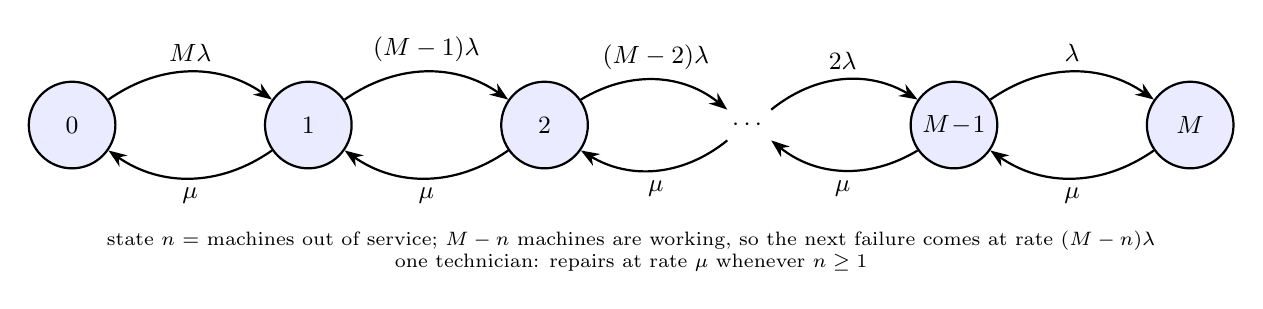
\begin{tikzpicture}[>=Stealth,font=\small,
 s/.style={draw,thick,circle,minimum size=1.1cm,inner sep=0pt,fill=blue!8},
 e/.style={->,thick},
 lab/.style={font=\small,fill=white,inner sep=1.5pt},
 every loop/.style={->,thick,looseness=6}]
\node[s] (0) at (0,0) {$0$};
\node[s] (1) at (3,0) {$1$};
\node[s] (2) at (6,0) {$2$};
\node (d) at (8.6,0) {$\cdots$};
\node[s] (M1) at (11.2,0) {$M\!-\!1$};
\node[s] (M) at (14.2,0) {$M$};
\foreach \a/\b/\r in {0/1/M\lambda,1/2/(M-1)\lambda,2/d/(M-2)\lambda,d/M1/2\lambda,M1/M/\lambda} {
  \draw[e] (\a) to[bend left=35] node[above]{$\r$} (\b);
  \draw[e] (\b) to[bend left=35] node[below]{$\mu$} (\a);
}
\node[font=\scriptsize,align=center] at (7.1,-1.6) {state $n$ = machines out of service; $M-n$ machines are working, so the next failure comes at rate $(M-n)\lambda$\\one technician: repairs at rate $\mu$ whenever $n\ge1$};
\end{tikzpicture}
\end{document}
